% =====================================================================
%  Neuro-Symbolic Causal Inference — Phase 1 (Machine Learning) Report
%  Compile:  tectonic Phase1_Report.tex      (or pdflatex twice / Overleaf)
%  Figures live in ./figures (regenerated from the project code).
% =====================================================================
\documentclass[11pt,a4paper]{article}

% ---------------------------------------------------------------- edit me
\newcommand{\MemberA}{Krishnadevan Manju Liby}
\newcommand{\MemberB}{Hemanth Tenneti}
\newcommand{\MemberC}{Arina Ali}
\newcommand{\MemberD}{Manan Bansal}
\newcommand{\MemberE}{Aaloke Eppalapalli}
\newcommand{\Institution}{Newton School of Technology, Rishihood University}
\newcommand{\Course}{CSAI Student Project --- Applied Machine Learning \& Deep Learning}
\newcommand{\RepoURL}{https://github.com/HemanthTenneti/AML-DL-Project-2026}
\newcommand{\ReportDate}{October 2026}

% ---------------------------------------------------------------- packages
\usepackage[T1]{fontenc}
\usepackage{amsmath,amssymb}
\usepackage{XCharter}
\usepackage[scale=0.93]{sourcesanspro}
\usepackage[xcharter,vvarbb]{newtxmath}
\usepackage[a4paper,top=2.5cm,bottom=2.4cm,left=2.4cm,right=2.4cm,headheight=14pt]{geometry}
\usepackage[table]{xcolor}
\usepackage{graphicx,booktabs,tabularx,array,multirow,enumitem,microtype}
\usepackage[nobottomtitles*]{titlesec}
\usepackage{fancyhdr,caption,subcaption,listings}
\renewcommand{\bottomtitlespace}{0.18\textheight}
\usepackage{tikz}
\usetikzlibrary{positioning,arrows.meta,calc,shapes.geometric,fit,backgrounds}
\usepackage[most]{tcolorbox}
\usepackage[hidelinks]{hyperref}
\usepackage[nameinlink,capitalise]{cleveref}

% ---------------------------------------------------------------- palette
% One colour per pipeline layer, used consistently in text, diagrams and plots.
\definecolor{ink}{HTML}{1B2A41}      % navy: text, headings
\definecolor{neural}{HTML}{6C4AB6}   % violet: language layer (text -> facts)
\definecolor{symbolic}{HTML}{0F8B8D} % teal: reasoning layer (PC + classifier)
\definecolor{causal}{HTML}{E07A2F}   % amber: graph layer (DAG, BN, do-queries)
\definecolor{mist}{HTML}{EEF1F5}
\definecolor{slate}{HTML}{5B6B7F}
\colorlet{neuralT}{neural!10}
\colorlet{symbolicT}{symbolic!10}
\colorlet{causalT}{causal!12}

\hypersetup{colorlinks=true,linkcolor=symbolic,citecolor=neural,urlcolor=causal}
\color{ink}

% ---------------------------------------------------------------- headings
\titleformat{\section}{\sffamily\Large\bfseries\color{ink}}
  {\tikz[baseline=(n.base)]\node[fill=symbolic,text=white,rounded corners=2pt,inner sep=4pt,minimum width=1.6em](n){\thesection};}{0.6em}{}
  [\vspace{-0.6em}{\color{symbolic!40}\rule{\linewidth}{0.6pt}}]
\titleformat{\subsection}{\sffamily\large\bfseries\color{ink}}{{\color{symbolic}\thesubsection}}{0.6em}{}
\titleformat{\subsubsection}{\sffamily\normalsize\bfseries\color{slate}}{}{0em}{}
\titlespacing*{\section}{0pt}{1.6em}{0.9em}
\titlespacing*{\subsection}{0pt}{1.2em}{0.4em}

% ---------------------------------------------------------------- header/footer
\pagestyle{fancy}\fancyhf{}
\renewcommand{\headrulewidth}{0pt}
\fancyhead[L]{\sffamily\small\color{slate}Neuro-Symbolic Causal Inference}
\fancyhead[R]{\sffamily\small\color{slate}Phase 1 Report \textbullet{} Project 1}
\fancyfoot[C]{\sffamily\small\color{slate}\thepage}
\fancyfoot[L]{\tikz{\fill[neural](0,0)rectangle(0.5,0.08);\fill[symbolic](0.5,0)rectangle(1,0.08);\fill[causal](1,0)rectangle(1.5,0.08);}}

% ---------------------------------------------------------------- captions, lists, tables
\captionsetup{font=small,labelfont={sf,bf,color=symbolic},labelsep=period,margin=0.5em}
\setlist{nosep,leftmargin=1.4em,topsep=0.3em}
\setlist[itemize]{label={\color{symbolic}\small$\blacktriangleright$}}
\renewcommand{\arraystretch}{1.18}
\newcommand{\thead}[1]{\leavevmode\sffamily\bfseries\color{white}#1}
\newcommand{\headrow}{\rowcolor{ink}}

% ---------------------------------------------------------------- boxes & chips
\newtcolorbox{keybox}[1][Key takeaway]{enhanced,breakable,colback=symbolicT,colframe=symbolic,
  boxrule=0pt,leftrule=3pt,arc=1pt,left=8pt,right=8pt,top=5pt,bottom=5pt,
  fonttitle=\sffamily\bfseries\small,coltitle=symbolic,colbacktitle=symbolicT,title=#1,
  attach title to upper={\ \ }}
\newtcolorbox{theorybox}[1]{enhanced,breakable,colback=white,colframe=ink!70,boxrule=0.5pt,arc=2pt,
  left=8pt,right=8pt,top=5pt,bottom=6pt,title={\sffamily\bfseries\small #1},colbacktitle=mist,coltitle=ink,
  toptitle=2pt,bottomtitle=2pt}
\newtcolorbox{examplebox}[1][]{enhanced,colback=mist,colframe=mist,arc=2pt,left=8pt,right=8pt,top=6pt,bottom=6pt,#1}
\newcommand{\chip}[2]{\tcbox[on line,colback=#1,colframe=#1,coltext=white,arc=2pt,boxsep=0pt,
  left=3pt,right=3pt,top=1.5pt,bottom=1.5pt,fontupper=\sffamily\bfseries\scriptsize]{#2}}
\newcommand{\LL}{\chip{neural}{LANGUAGE}}
\newcommand{\RL}{\chip{symbolic}{REASONING}}
\newcommand{\GL}{\chip{causal}{GRAPH}}
\newcommand{\code}[1]{\texttt{\small\color{neural!80!black}#1}}
\newcommand{\doop}{\mathrm{do}}

\lstset{basicstyle=\ttfamily\footnotesize,keywordstyle=\color{neural}\bfseries,commentstyle=\color{slate}\itshape,
  stringstyle=\color{causal!80!black},backgroundcolor=\color{mist},frame=none,xleftmargin=6pt,framexleftmargin=6pt,
  aboveskip=6pt,belowskip=6pt,columns=fullflexible,keepspaces=true,showstringspaces=false,language=Python}

% =====================================================================
\begin{document}

% ---------------------------------------------------------------- title page
\begin{titlepage}
\thispagestyle{empty}
\begin{tikzpicture}[remember picture,overlay]
  \fill[ink] (current page.north west) rectangle ([yshift=-12.2cm]current page.north east);
  \fill[neural]   ([yshift=-12.2cm]current page.north west) rectangle ([xshift=7cm,yshift=-12.5cm]current page.north west);
  \fill[symbolic] ([xshift=7cm,yshift=-12.2cm]current page.north west) rectangle ([xshift=14cm,yshift=-12.5cm]current page.north west);
  \fill[causal]   ([xshift=14cm,yshift=-12.2cm]current page.north west) rectangle ([yshift=-12.5cm]current page.north east);
  % decorative causal graph in the banner
  \begin{scope}[shift={([xshift=-5.3cm,yshift=-4.2cm]current page.north east)},
      every node/.style={circle,minimum size=0.95cm,font=\sffamily\bfseries,text=white,line width=1.2pt},
      arr/.style={-{Stealth[length=2.6mm]},line width=1.1pt,white!70!ink}]
    \node[fill=neural]   (A) at (0,1.2)  {A};
    \node[fill=symbolic] (B) at (2.6,1.6){B};
    \node[fill=symbolic] (C) at (1.2,-0.4){C};
    \node[fill=causal]   (D) at (3.6,-0.2){D};
    \node[fill=neural]   (E) at (0.2,-2.2){E};
    \node[fill=causal]   (F) at (2.8,-2.4){F};
    \draw[arr] (A)--(C); \draw[arr] (B)--(C); \draw[arr] (B)--(D); \draw[arr] (C)--(F);
    \draw[arr] (D)--(F); \draw[arr] (C)--(E);
    \draw[white!45!ink,dashed,line width=1pt] (A)--(E);
  \end{scope}
  \node[anchor=north west,text width=11cm,align=left] at ([xshift=2.4cm,yshift=-2.3cm]current page.north west)
    {\sffamily\small\bfseries\color{causal}PROJECT 1 \textbullet{} CAUSAL NLP REASONING};
  \node[anchor=north west,text width=11.2cm,align=left] at ([xshift=2.4cm,yshift=-3.2cm]current page.north west)
    {\sffamily\fontsize{30}{34}\selectfont\bfseries\color{white}Neuro-Symbolic\\Causal Inference};
  \node[anchor=north west,text width=11.6cm,align=left] at ([xshift=2.4cm,yshift=-6.15cm]current page.north west)
    {\sffamily\large\hyphenpenalty=10000\color{white!80!ink}via Language-Model Knowledge Extraction and Bayesian Networks};
  \node[anchor=north west,text width=11cm,align=left] at ([xshift=2.4cm,yshift=-8.4cm]current page.north west)
    {\tcbox[on line,colback=white,colframe=white,arc=2pt,boxsep=0pt,left=6pt,right=6pt,top=4pt,bottom=4pt,
      fontupper=\sffamily\bfseries\small\color{ink}]{PHASE 1 \;\textbar\; MACHINE LEARNING EVALUATION}};
  \node[anchor=north west,text width=11cm,align=left] at ([xshift=2.4cm,yshift=-9.6cm]current page.north west)
    {\sffamily\small\color{white!70!ink}Project Report \textbullet{} \ReportDate};
\end{tikzpicture}

\vspace*{11.4cm}
\begin{center}
\begin{minipage}{0.86\textwidth}\sffamily
\begin{tabularx}{\linewidth}{@{}>{\leavevmode\bfseries\color{slate}\small}p{3.3cm}X@{}}
SUBMITTED BY & \MemberA \\ & \MemberB \\ & \MemberC \\ & \MemberD \\ & \MemberE \\[0.6em]
INSTITUTION  & \Institution \\[0.3em]
COURSE       & \Course \\[0.3em]
DATASET      & Corr2Cause (Jin et al., ICLR 2024), corrected labels \\[0.3em]
REPOSITORY   & \small\url{\RepoURL}
\end{tabularx}
\end{minipage}

\vfill
\begin{minipage}{0.86\textwidth}\sffamily\small
{\color{slate}\bfseries COLOUR KEY USED THROUGHOUT THIS REPORT}\\[0.4em]
\LL\ text $\rightarrow$ facts \qquad \RL\ facts $\rightarrow$ valid claims \qquad \GL\ claims $\rightarrow$ DAG $\rightarrow$ what-if
\end{minipage}
\end{center}
\end{titlepage}

% ---------------------------------------------------------------- abstract + contents
\setcounter{page}{2}
\begin{tcolorbox}[enhanced,colback=mist,colframe=mist,arc=2pt,left=12pt,right=12pt,top=10pt,bottom=10pt]
{\sffamily\bfseries\large Abstract}\par\smallskip
Language models are good at sounding causal and bad at \emph{being} causal: given a list of
correlations, they often claim causes that the data cannot support. This project separates the two jobs.
A \emph{language layer} turns text into structured statistical facts; a \emph{reasoning layer} applies
textbook causal-discovery rules (the PC algorithm) and an interpretable classifier to decide which causal
claims are actually entailed; a \emph{graph layer} assembles the accepted cause$\rightarrow$effect triples
into an acyclic graph, fits a Bayesian network with \texttt{pgmpy}, and answers intervention queries.

In Phase~1 every layer is classical machine learning. On the Corr2Cause benchmark our
Rules\,+\,PC\,+\,Decision-Tree pipeline reaches an F1 of \textbf{0.997} on the held-out test set
(text-only TF-IDF baseline: 0.655), stays at \textbf{0.997} when all variable names are changed
(baseline: 0.322), recovers \textbf{73/73} gold cause edges with no false edges, and answers
\textbf{97.5\%} of 242 known intervention queries correctly. An ablation shows that the reasoning
features, not the wording, carry the signal. The one clear failure, \emph{paraphrased} hypotheses that the
hand-written rules cannot read (F1 = 0), is the gap that Phase~2 targets with DistilBERT.
\end{tcolorbox}

\vspace{0.8em}
{\sffamily
\setcounter{tocdepth}{1}
\renewcommand{\contentsname}{\large Contents}
\tableofcontents}

\newpage
% =====================================================================
\section{Introduction}

News articles and scientific abstracts are full of statements such as ``X is associated with Y''.
Turning such statements into reliable \emph{causal} conclusions is hard, and it is exactly where
large language models stumble: on the Corr2Cause benchmark, which asks whether a causal claim follows
from a set of correlations, the original study found that even strong fine-tuned transformers mostly
pattern-match and fall apart when the wording or variable names change~\cite{jin2024corr2cause}.

The project brief asks for a system that \emph{extracts candidate cause--effect relations from text and
then represents and tests them in a Bayesian network}, keeping ``fluent language understanding'' separate
from ``formal causal reasoning and counterfactual queries''. We take that separation literally and build a
three-layer pipeline with fixed interfaces, so that Phase~2 can replace a single layer and be compared
fairly with Phase~1.

\begin{figure}[!htbp]
\centering
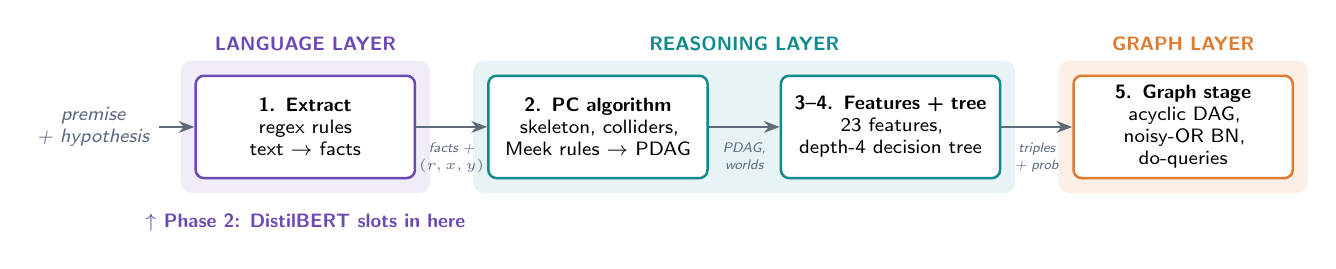
\begin{tikzpicture}[
  stage/.style={draw=#1,fill=white,rounded corners=3pt,line width=0.9pt,minimum height=1.3cm,
                text width=2.55cm,align=center,font=\sffamily\scriptsize,execute at begin node=\hyphenpenalty 10000\relax},
  data/.style={font=\sffamily\tiny\itshape,text=slate,align=center},
  flow/.style={-{Stealth[length=2mm]},line width=0.9pt,ink!70},
  node distance=0.9cm]
  \node[stage=neural]   (s1) {\textbf{1. Extract}\\regex rules\\text $\rightarrow$ facts};
  \node[stage=symbolic, right=of s1] (s2) {\textbf{2. PC algorithm}\\skeleton, colliders,\\Meek rules $\rightarrow$ PDAG};
  \node[stage=symbolic, right=of s2] (s3) {\textbf{3--4. Features + tree}\\23 features,\\depth-4 decision tree};
  \node[stage=causal,   right=of s3] (s5) {\textbf{5. Graph stage}\\acyclic DAG,\\noisy-OR BN, do-queries};
  \node[data,left=0.45cm of s1,font=\sffamily\scriptsize\itshape] (txt) {premise\\+ hypothesis};
  \draw[flow] (txt)--(s1); \draw[flow] (s1)--(s2); \draw[flow] (s2)--(s3); \draw[flow] (s3)--(s5);
  \node[data,below=0.08cm of $(s1.east)!0.5!(s2.west)$] {facts +\\$(r,x,y)$};
  \node[data,below=0.08cm of $(s2.east)!0.5!(s3.west)$] {PDAG,\\worlds};
    \node[data,below=0.08cm of $(s3.east)!0.5!(s5.west)$] {triples\\+ prob};
  \begin{scope}[on background layer]
    \node[fit=(s1),fill=neuralT,rounded corners=4pt,inner sep=5pt,label={[font=\sffamily\scriptsize\bfseries,text=neural]above:LANGUAGE LAYER}] {};
    \node[fit=(s2)(s3),fill=symbolicT,rounded corners=4pt,inner sep=5pt,label={[font=\sffamily\scriptsize\bfseries,text=symbolic]above:REASONING LAYER}] {};
    \node[fit=(s5),fill=causalT,rounded corners=4pt,inner sep=5pt,label={[font=\sffamily\scriptsize\bfseries,text=causal]above:GRAPH LAYER}] {};
  \end{scope}
  \node[font=\sffamily\scriptsize\bfseries,text=neural,below=0.32cm of s1] {$\uparrow$ Phase 2: DistilBERT slots in here};
\end{tikzpicture}
\caption{The Phase~1 pipeline. Each layer has one job and a fixed interface. The language layer is the only
part Phase~2 will replace, so the reasoning and graph layers (and the evaluation code) stay identical.}
\label{fig:pipeline}
\end{figure}

\paragraph{Contributions of Phase 1.}
\begin{itemize}
  \item A transparent, end-to-end ML pipeline that goes from raw text to intervention answers (\cref{fig:pipeline}).
  \item An implementation of the PC orientation rules plus enumeration of \emph{equivalent DAGs}, giving a
        ``support'' feature that measures how many causal worlds agree with a claim.
  \item A feature ablation, a text-only baseline, and two robustness tests (renamed variables, reworded hypotheses).
  \item A graph stage that enforces acyclicity, quantifies effects with a Bayesian network, and shows numerically
        why correlation and intervention differ.
  \item A reproducible repository with unit tests and an interactive pipeline tracer (\cref{sec:repro}).
\end{itemize}

\begin{table}[!htbp]
\centering\small
\caption{Where each Phase~1 evaluation criterion is addressed.}
\label{tab:rubric}
\begin{tabularx}{0.92\linewidth}{@{}lX@{}}
\headrow \thead{Criterion} & \thead{Section(s)} \\
Literature review & \cref{sec:lit} \\
\rowcolor{mist} Dataset quality \& EDA & \cref{sec:data} (splits, leakage check, label correction, class balance) \\
Feature engineering & \cref{sec:features} (23 features in 4 groups) and the ablation in \cref{sec:ablation} \\
\rowcolor{mist} Theoretical rigour & \cref{sec:theory} (Markov equivalence, support criterion, do-calculus) \\
Model application & \cref{sec:results,sec:graph} \\
\rowcolor{mist} GitHub repository \& code quality & \cref{sec:repro} \\
\end{tabularx}
\end{table}

% =====================================================================
\section{Background and Literature Review}\label{sec:lit}

\subsection{Causal reasoning with graphs}
Pearl's work on Bayesian networks~\cite{pearl1988} gave a compact way to encode a joint distribution as a
directed acyclic graph (DAG) plus local conditional probability tables, with \emph{d-separation} linking graph
structure to conditional independence. \emph{Causality}~\cite{pearl2009} added the $\doop(\cdot)$ operator:
$P(Y \mid \doop(X{=}x))$ is what happens when we \emph{set} $X$, which can differ sharply from
$P(Y \mid X{=}x)$, what we see when we merely \emph{observe} it.

\subsection{Causal discovery from independence facts}
If all conditional independences of a system are known, the PC algorithm~\cite{spirtes2000} recovers the
graph's \emph{skeleton} and the direction of every edge that the data can identify. Verma and
Pearl~\cite{verma1990} showed that two DAGs are indistinguishable from observational data exactly when they
share a skeleton and their v-structures (colliders $X\!\rightarrow\!Z\!\leftarrow\!Y$); Meek~\cite{meek1995}
gave the complete set of rules for orienting the remaining edges. The output is a partially directed graph
(PDAG) that stands for a whole \emph{Markov equivalence class} of DAGs.

\subsection{Causal relations in text and the Corr2Cause benchmark}
Classical causal relation extraction relies on lexical and dependency patterns (``X leads to Y'', ``due to'')~\cite{khoo2000,girju2003};
it is precise on the templates it knows and blind to everything else. Transformers such as BERT~\cite{devlin2019}
and its distilled version DistilBERT~\cite{sanh2019} learn wording from data and are now standard for relation
classification. Corr2Cause~\cite{jin2024corr2cause} tests whether such models can \emph{reason}: each premise lists
every correlation and independence in a small closed system, and the model must judge whether a causal hypothesis
is entailed. The authors report that off-the-shelf LLMs score near chance and that fine-tuned models fail under
paraphrasing and variable renaming, a classic case of shortcut learning~\cite{gururangan2018,geirhos2020}.
Surveys of LLM causal reasoning reach a similar conclusion: fluent causal language is not the same as causal
inference~\cite{kiciman2023}.

\subsection{Positioning}
Neuro-symbolic AI argues for pairing learned perception with explicit reasoning~\cite{garcez2023}. Our design
follows this line (\cref{tab:lit}): the language layer handles wording, while acyclicity, uncertainty and
interventions are guaranteed by symbolic machinery rather than hoped for from a text model.

\begin{table}[!htbp]
\centering\small
\caption{How the main approaches compare, and what we take from each.}
\label{tab:lit}
\begin{tabularx}{\linewidth}{@{}>{\raggedright}p{3.1cm}>{\raggedright}X>{\raggedright\arraybackslash}X@{}}
\headrow \thead{Approach} & \thead{Strength} & \thead{Limitation / our use} \\
Pattern-based extraction~\cite{khoo2000,girju2003} & Precise, explainable & Brittle to rewording. \emph{Our Phase~1 language layer.} \\
\rowcolor{mist} PC algorithm + Meek rules~\cite{spirtes2000,meek1995} & Provably sound orientation & Needs independence facts as input. \emph{Our reasoning core.} \\
Bayesian networks, do-calculus~\cite{pearl1988,pearl2009} & Uncertainty and interventions & Needs a DAG. \emph{Our graph layer (pgmpy~\cite{ankan2015}).} \\
\rowcolor{mist} End-to-end transformers~\cite{devlin2019,sanh2019} & Robust to wording & Shortcut-prone at reasoning~\cite{jin2024corr2cause}. \emph{Phase~2 language layer.} \\
\end{tabularx}
\end{table}

% =====================================================================
\section{Dataset and Exploratory Analysis}\label{sec:data}

\subsection{Corr2Cause in one example}
Each row pairs a \emph{premise} (all statistical relations in a closed system of 2--6 variables) with one
\emph{hypothesis} and a binary label: 1 if the claim \emph{must} hold, 0 otherwise. A real test example:

\begin{examplebox}
\small\textbf{Premise.} Suppose there is a closed system of 3 variables, A, B and C. All the statistical relations
among these 3 variables are as follows: A correlates with C. B correlates with C. However, A is independent of B.\\[0.3em]
\textbf{Hypotheses.} ``A directly causes C.'' \chip{symbolic}{label 1} \quad
``B directly causes A.'' \chip{slate}{label 0} \quad
``There exists at least one collider of B and C.'' \chip{slate}{label 0}
\end{examplebox}

The reasoning: A and C are dependent, B and C are dependent, but A and B are independent. The only structure
consistent with this is the collider $A\rightarrow C\leftarrow B$, so ``A directly causes C'' is entailed.

We chose Corr2Cause, the starter dataset the brief recommends, because every label is
\emph{provably} correct with respect to the premise. That lets us measure extraction and reasoning exactly,
which is not possible with open news text, where the ``true'' causal graph is unknown.

\subsection{Splits, robustness sets and leakage}
\Cref{tab:splits} summarises the data. Many hypotheses share a premise, so a random row split would leak
near-duplicate text between train and test. Following the brief (``split documents before extraction''), we
use the official \textbf{premise-grouped} split and verified that train and test share \textbf{0 premises}.
Dev shares 2 of its 22 premises with train, so we treat dev as a secondary check and report headline numbers on test.

Two official robustness sets reuse the 21 test premises: \emph{refactorization} renames variables
(e.g.\ A, B and C become Z, Y and X) and \emph{paraphrase} rewords the hypotheses
(``directly causes'' $\rightarrow$ ``directly affects'').

\begin{table}[!htbp]
\centering\small
\caption{Data used in Phase~1 (corrected labels).}
\label{tab:splits}
\begin{tabular}{@{}lrrrl@{}}
\headrow \thead{Split} & \thead{Rows} & \thead{Premises} & \thead{\% valid} & \thead{Purpose} \\
train            & 205{,}734 & 2{,}338 & 21.0 & fit all models \\
\rowcolor{mist} dev & 1{,}076 & 22 & 14.8 & secondary check \\
test             & 1{,}162 & 21 & 16.5 & headline results \\
\rowcolor{mist} refactorization & 2{,}246 & 21 & 16.2 & robustness: renamed variables \\
paraphrase       & 2{,}246 & 21 & 16.2 & robustness: reworded hypotheses \\
\end{tabular}
\end{table}

\subsection{Label quality}
The original Corr2Cause generator contained a bug that wrote 6{,}943 wrong labels (3.3\%). We use the
publicly released corrected labels~\cite{corr2causecorrected}, which keep the text identical. The fix changes
6{,}897 train, 28 dev and 18 test labels. We noticed the problem ourselves when our PC reasoner kept
``disagreeing'' with the original labels on whole premises; for transparency, \cref{sec:results} also
reports test scores on the original labels.

\subsection{What the data looks like}
\begin{figure}[!htbp]
\centering
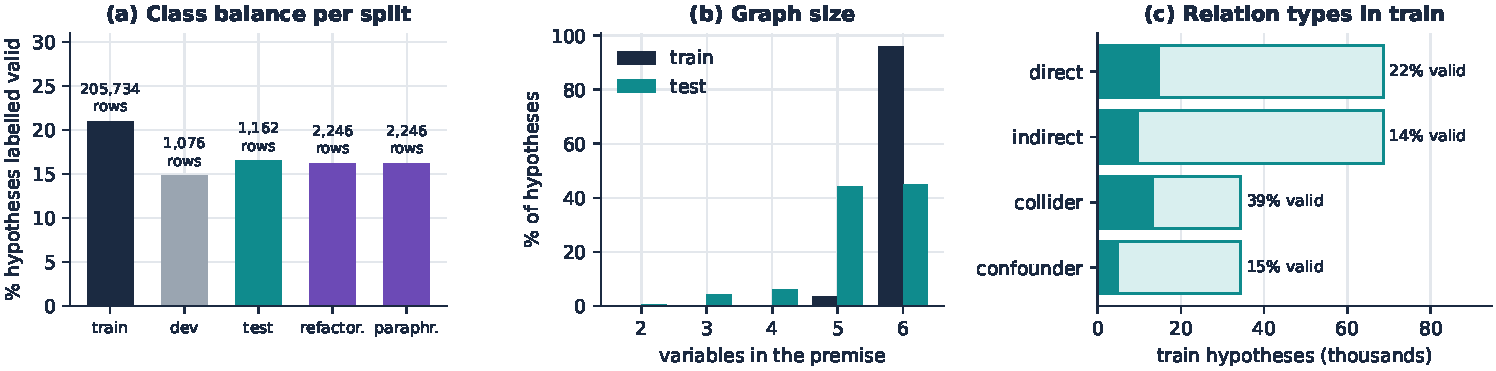
\includegraphics[width=\linewidth]{figures/fig_eda.pdf}
\caption{(a) Only 15--21\% of hypotheses are valid in every split, so we report F1 of the valid class rather than accuracy.
(b) Training premises are almost all 6-variable systems, while test spans 2--6 variables: a mild distribution
shift that rewards methods that generalise across graph sizes. (c) Each premise is asked about every relation type
for every variable pair; collider claims are valid far more often than the others.}
\label{fig:eda}
\end{figure}

Three EDA findings shaped the design:
\begin{itemize}
  \item \textbf{Imbalance.} A model that always says ``not valid'' gets about 84\% accuracy on test, which is
        meaningless. F1 of the valid class is the primary metric throughout.
  \item \textbf{Size shift.} Train is dominated by 6-variable graphs, test is not. Features that depend on
        graph \emph{structure} rather than raw counts should transfer better.
  \item \textbf{Names carry order.} Variables are lettered in causal order in the generator, so ``a later letter
        causes an earlier one'' is nearly always false. A text model can exploit this shortcut, and the
        refactorization set exists to catch it.
\end{itemize}

% =====================================================================
\section{Theoretical Foundations}\label{sec:theory}

This section collects the theory the pipeline relies on. Each result is short, but together they explain why the
system is correct by construction rather than by luck.

\begin{theorybox}{T1 \quad Faithfulness and the skeleton}
In a faithful causal DAG, two variables $X,Y$ are \emph{adjacent} if and only if no set $S$ of other variables
makes them conditionally independent ($X \not\!\perp\!\!\!\perp Y \mid S$ for all $S$). Corr2Cause lists every
independence, so the skeleton is read off directly: join $X$ and $Y$ when they have no separating set.
\end{theorybox}

\begin{theorybox}{T2 \quad Colliders are identifiable; most other edges are not}
For a path $X - Z - Y$ with $X,Y$ non-adjacent, $Z$ is a collider ($X\!\rightarrow\!Z\!\leftarrow\!Y$) iff $Z$
belongs to \emph{no} separating set of $(X,Y)$. Two DAGs are observationally equivalent iff they share the skeleton and
the v-structures~\cite{verma1990}. Meek's rules R1--R3~\cite{meek1995} then orient every edge whose reversal would
create a cycle or a new collider. Edges still undirected after that are genuinely unidentifiable.
\end{theorybox}

\begin{theorybox}{T3 \quad The validity criterion (``support'')}
Let $\mathcal{E}(G)$ be the set of DAGs represented by the PDAG $G$. For a hypothesis $h$ (e.g.\ ``$X$ directly causes $Y$''),
\[
  \operatorname{supp}(h) \;=\; \frac{1}{|\mathcal{E}(G)|}\sum_{D\in\mathcal{E}(G)} \mathbb{1}\!\left[\,h \text{ holds in } D\,\right].
\]
Corr2Cause labels a claim valid iff it is implied by the premise, i.e.\ true in \emph{every} equivalent DAG, so
$h$ is valid $\Leftrightarrow \operatorname{supp}(h)=1$. A claim with support $0.67$ is \emph{possible} but not \emph{entailed}.
\end{theorybox}

\begin{theorybox}{T4 \quad Interventions in a Bayesian network}
A DAG with conditional tables factorises as $P(v_1,\dots,v_n)=\prod_i P(v_i\mid \mathrm{pa}_i)$. Setting $X{=}x$
deletes $X$'s own factor (\emph{truncated factorisation}~\cite{pearl2009}):
$P(\mathbf{v}\mid\doop(X{=}x))=\prod_{i:V_i\neq X}P(v_i\mid\mathrm{pa}_i)\big|_{X=x}$.
We report the average causal effect $\mathrm{ACE}=P(Y{=}1\mid\doop(X{=}1))-P(Y{=}1\mid\doop(X{=}0))$.
When $X$ and $Y$ share a cause $Z$, the observational difference $P(Y\mid X{=}1)-P(Y\mid X{=}0)$ also contains
the $X\leftarrow Z\rightarrow Y$ path and therefore overstates the effect (\cref{sec:do}).
\end{theorybox}

% =====================================================================
\section{Methodology}\label{sec:method}

\subsection{Stage 1: Text to facts \texorpdfstring{\quad\LL}{}}
We first fixed a small \textbf{entity schema}. Variables are single capital letters, and
premise facts take two forms, \code{correlates(X,Y)} and \code{independent(X,Y|S)}. Hypotheses are one of four relations
(\cref{tab:schema}). One regular expression per sentence template fills this schema. Every fact keeps
its premise id, and self-loops ($X$ causes $X$) are rejected.

\begin{table}[!htbp]
\centering\small
\caption{The four causal relation types (our entity schema).}
\label{tab:schema}
\begin{tabular}{@{}lll@{}}
\headrow \thead{Relation} & \thead{Template wording} & \thead{Meaning in a DAG} \\
direct     & ``X directly causes Y.'' & $X\rightarrow Y$ \\
\rowcolor{mist} indirect & ``X causes something else which causes Y.'' & $X\rightarrow Z\rightarrow\cdots\rightarrow Y$ \\
collider   & ``There exists at least one collider of X and Y.'' & $X\rightarrow\cdots\rightarrow Z\leftarrow\cdots\leftarrow Y$ \\
\rowcolor{mist} confounder & ``There exists at least one confounder of X and Y.'' & $X\leftarrow\cdots\leftarrow Z\rightarrow\cdots\rightarrow Y$ \\
\end{tabular}
\end{table}

\begin{lstlisting}
HYPOTHESIS_PATTERNS = [   # src/causal_nlp/parsing.py  (one rule per template)
    (re.compile(rf"^{VAR} directly causes {VAR}\.$"), DIRECT, 1, 2),
    (re.compile(rf"^{VAR} causes something else which causes {VAR}\.$"), INDIRECT, 1, 2),
    ...
]
def parse_hypothesis(text) -> Hypothesis | None:   # None = "unseen wording"
\end{lstlisting}

The parser returns a typed \code{Hypothesis(relation, x, y)} or \code{None}. This tiny interface is the
contract Phase~2 must honour: a DistilBERT parser only needs to return the same tuple.

\subsection{Stage 2: Facts to a causal graph \texorpdfstring{\quad\RL}{}}
We implemented the three PC steps directly on the extracted facts (T1--T2): build the skeleton, orient
v-structures, then apply Meek rules R1--R3 until nothing changes. To evaluate a hypothesis we then enumerate the
equivalent DAGs: flip every undirected edge both ways and keep the combinations with no cycle and no extra
collider. \Cref{fig:pdag} shows a real test premise with two undirected edges, giving $2^2=4$ candidate
orientations, of which 3 are valid DAGs.

\begin{figure}[!htbp]
\centering
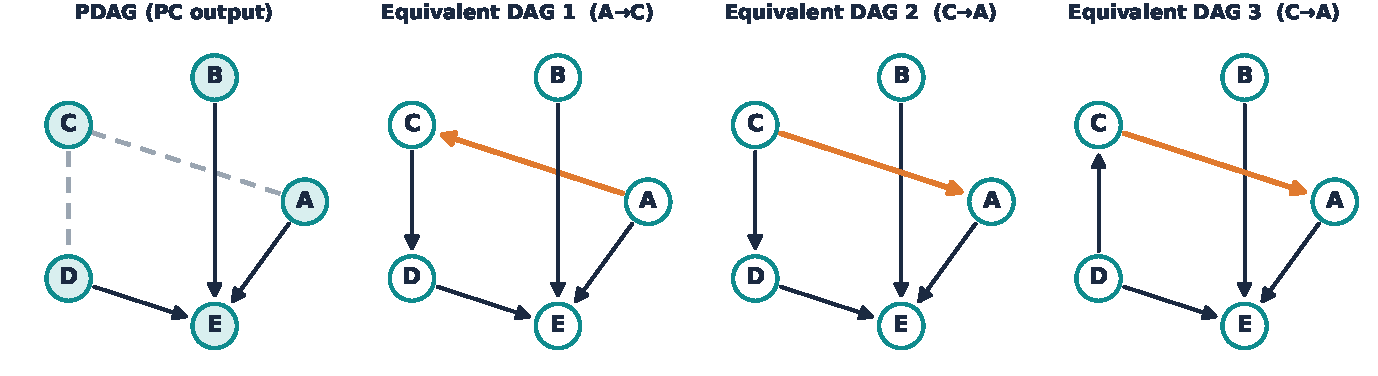
\includegraphics[width=\linewidth]{figures/fig_pdag.pdf}
\caption{A 5-variable test premise. Left: the PDAG produced by our PC implementation (dashed = direction unknown).
Right: its three equivalent DAGs. The edge between A and C points A$\rightarrow$C in only one of them, so
$\operatorname{supp}(\text{A directly causes C}) = 1/3$ and the claim is \emph{not} valid. By contrast,
``C is an indirect cause of E'' holds in all three worlds (support 1.0) and is valid.}
\label{fig:pdag}
\end{figure}

\subsection{Stage 3: Feature engineering}\label{sec:features}
Each (premise, hypothesis) pair becomes a row of 23 numbers in four groups (\cref{tab:features}). The groups
mirror the reasoning steps, which lets the ablation measure how much each step adds. One design rule matters
for robustness: \textbf{no feature uses a variable's name}, so renaming variables cannot change any input.

\begin{table}[!htbp]
\centering\small
\caption{Engineered features. Group colours follow the pipeline layers.}
\label{tab:features}
\begin{tabularx}{\linewidth}{@{}lcX@{}}
\headrow \thead{Group} & \thead{\#} & \thead{Features (intuition)} \\
Relation & 4 & one-hot of the claimed relation \hfill \emph{what is being claimed} \\
\rowcolor{mist} \textcolor{neural}{\textbf{Text facts}} & 8 & no.\ of variables; $X$--$Y$ correlated; adjacent in skeleton; no.\ of separating sets; size of smallest separating set; degree of $X$, $Y$; common neighbours \hfill \emph{read straight off the sentences} \\
\textcolor{symbolic}{\textbf{PC graph}} & 9 & $X\!\rightarrow\!Y$, $Y\!\rightarrow\!X$, undirected; $X$ ancestor of $Y$ (definite / possible) and reverse; common children; common parents \hfill \emph{read off the PDAG} \\
\rowcolor{mist} \textcolor{symbolic}{\textbf{Support}} & 2 & $\operatorname{supp}(h)$; number of equivalent DAGs \hfill \emph{how many possible worlds agree} \\
\end{tabularx}
\end{table}

Building features for all 212{,}464 rows takes about 12\,s on a laptop CPU, because each premise is parsed and
analysed once and cached across its hypotheses.

\subsection{Stage 4: Classifiers}
\begin{itemize}
  \item \textbf{Text-only baseline: TF-IDF + logistic regression.} Word 1--3-grams of premise and hypothesis
        (one-letter tokens kept so variable names are visible), class-balanced loss. No parsing and no reasoning.
        This is the fair ML counterpart of an end-to-end transformer.
  \item \textbf{Feature models:} logistic regression (standardised), a \textbf{depth-4 decision tree}, and a
        300-tree random forest, each trained on the three cumulative feature groups.
\end{itemize}
We chose the decision tree as the final model. It matches the forest's accuracy, it can be printed and checked by
hand, and it outputs a probability that the graph stage uses as an edge confidence. All models use seed 42.

\subsection{Stage 5: From triples to answers \texorpdfstring{\quad\GL}{}}
Only claims the classifier marks valid (\code{prob\,$\ge$\,0.5}) reach the graph stage, which is how we implement
the brief's ``feed only reviewed predictions into the graph stage''.
\begin{enumerate}[label=\textcolor{causal}{\textbf{\arabic*.}}]
  \item \textbf{Acyclic DAG.} Predicted \emph{direct} edges are added from most to least confident; an edge that
        would close a cycle, or is a self-loop, is rejected and logged.
  \item \textbf{Bayesian network.} Corr2Cause provides structure but no measurements, so each node receives
        illustrative \emph{noisy-OR} tables: $P(V{=}1\mid k \text{ active parents}) = 1-(1-0.1)(1-0.7)^{k}$
        (base rate 10\%, each cause fires with 70\%). The network is built and checked in \texttt{pgmpy}~\cite{ankan2015}.
  \item \textbf{Intervention queries.} For each query ``does $\doop(X)$ change $Y$?'' we compute the ACE (T4) with
        \texttt{CausalInference} and answer ``yes'' if $\mathrm{ACE}>0.01$.
\end{enumerate}
\emph{Known} queries are those whose answer is fixed by the gold labels or the text: \emph{yes} if $X$ directly or
indirectly causes $Y$; \emph{no} if $Y$ causes $X$ (an effect cannot cause its cause) or if $X$ and $Y$ are not even correlated.

% =====================================================================
\section{Experiments and Results}\label{sec:results}

\paragraph{Protocol.} All models are trained on the full train split and evaluated on the untouched test set. The
primary metric is \textbf{F1 of the valid class}; we also report precision and recall. Nothing is tuned on test.

\subsection{Ablation: reasoning, not wording, carries the signal}\label{sec:ablation}

\begin{figure}[!htbp]
\centering
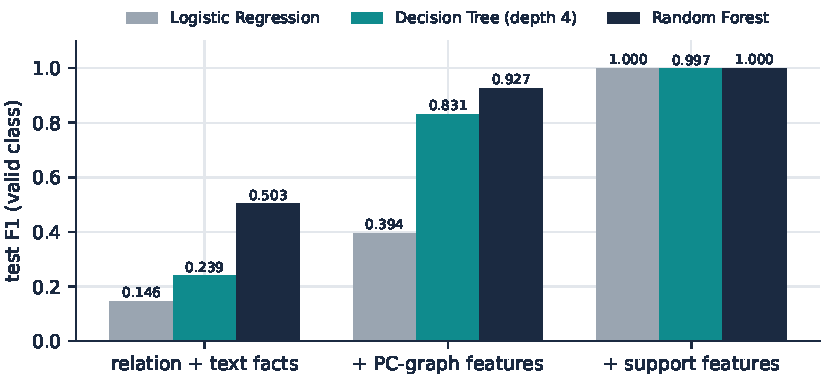
\includegraphics[width=0.86\linewidth]{figures/fig_ablation.pdf}
\caption{Test F1 as feature groups are added. Text facts alone are weak; PC-graph features give the largest jump;
support makes the task essentially solved for every model.}
\label{fig:ablation}
\end{figure}

\Cref{fig:ablation} tells the main story of Phase~1. With only facts read off the sentences, even a random forest
reaches F1 of just 0.50, because validity depends on \emph{combinations} of facts that a flat model cannot form. Adding the
PC-graph features lifts the tree from 0.24 to 0.83 and the forest to 0.93. Adding support takes all three models to
0.997--1.000. Once the reasoning is done symbolically, the learning problem becomes almost linearly separable.

\subsection{The final model is a readable rule}
\begin{figure}[!htbp]
\centering
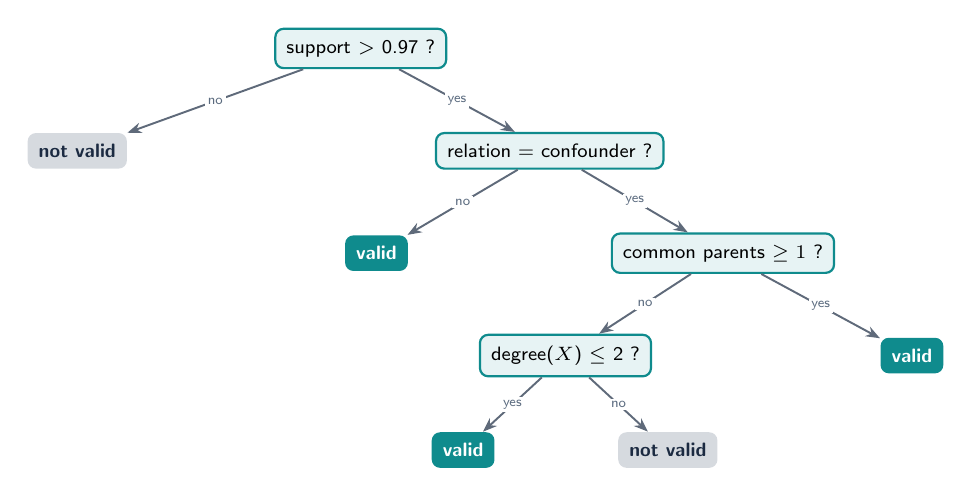
\begin{tikzpicture}[
  q/.style={draw=symbolic,fill=symbolicT,rounded corners=3pt,font=\sffamily\scriptsize,align=center,inner sep=4pt,line width=0.8pt},
  yes/.style={fill=symbolic,text=white,rounded corners=3pt,font=\sffamily\scriptsize\bfseries,inner sep=4pt},
  no/.style={fill=slate!25,text=ink,rounded corners=3pt,font=\sffamily\scriptsize\bfseries,inner sep=4pt},
  e/.style={-{Stealth[length=1.8mm]},ink!70,line width=0.7pt},
  lab/.style={font=\sffamily\tiny,text=slate,midway,fill=white,inner sep=1pt}]
  \node[q] (r) at (0,0) {support $>$ 0.97 ?};
  \node[no] (n1) at (-3.6,-1.3) {not valid};
  \node[q]  (c) at (2.4,-1.3) {relation = confounder ?};
  \node[yes](y1) at (0.2,-2.6) {valid};
  \node[q]  (p) at (4.6,-2.6) {common parents $\ge 1$ ?};
  \node[yes](y2) at (7.0,-3.9) {valid};
  \node[q]  (d) at (2.6,-3.9) {degree($X$) $\le$ 2 ?};
  \node[yes](y3) at (1.3,-5.1) {valid};
  \node[no] (n2) at (3.9,-5.1) {not valid};
  \draw[e] (r)--node[lab]{no}(n1); \draw[e] (r)--node[lab]{yes}(c);
  \draw[e] (c)--node[lab]{no}(y1); \draw[e] (c)--node[lab]{yes}(p);
  \draw[e] (p)--node[lab]{yes}(y2); \draw[e] (p)--node[lab]{no}(d);
  \draw[e] (d)--node[lab]{yes}(y3); \draw[e] (d)--node[lab]{no}(n2);
\end{tikzpicture}
\caption{The learned depth-4 tree, simplified (the left subtree's three leaves all predict ``not valid''). The tree
\emph{learned} the rule ``valid iff support $\approx 1$'' from data, plus a small branch for confounders that absorbs a
quirk in how the generator defines a common cause.}
\label{fig:tree}
\end{figure}

The tree in \cref{fig:tree} rediscovers criterion T3 on its own, without being told. Support accounts for 99\% of its
Gini importance (\cref{fig:treeeval}a). The test confusion matrix (\cref{fig:treeeval}b) has exactly one error: a valid
\emph{confounder} claim the confounder branch rejects, giving confounder recall 0.93 (14 of 15). All other relations score
F1 = 1.00.

\begin{figure}[!htbp]
\centering
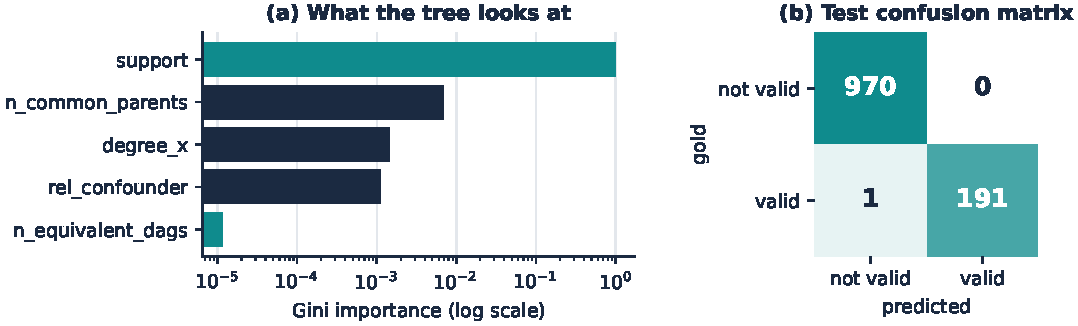
\includegraphics[width=0.92\linewidth]{figures/fig_tree_eval.pdf}
\caption{(a) Feature importance of the final tree (log scale). (b) Test confusion matrix: 970 true negatives,
191 true positives, 0 false positives, 1 false negative.}
\label{fig:treeeval}
\end{figure}

\subsection{Comparison and robustness}

\begin{table}[!htbp]
\centering\small
\caption{Relation-extraction results, F1 of the valid class (precision / recall below each F1 on test).}
\label{tab:main}
\begin{tabular}{@{}lccccc@{}}
\headrow \thead{System} & \thead{dev} & \thead{test} & \thead{refactor.} & \thead{paraphrase} & \thead{test, orig.\ labels} \\
TF-IDF + LR (text only) & 0.606 & 0.655 & 0.322 & 0.250 & 0.625 \\
\multicolumn{1}{r}{\scriptsize\color{slate}P / R} & & \scriptsize\color{slate}0.50 / 0.94 & \scriptsize\color{slate}0.49 / 0.24 & \scriptsize\color{slate}0.27 / 0.23 & \\
\rowcolor{symbolicT} \textbf{Rules + PC + Decision Tree} & \textbf{1.000} & \textbf{0.997} & \textbf{0.997} & 0.000 & \textbf{0.949} \\
\rowcolor{symbolicT} \multicolumn{1}{r}{\scriptsize\color{slate}P / R} & & \scriptsize\color{slate}1.00 / 0.99 & \scriptsize\color{slate}1.00 / 0.99 & \scriptsize\color{slate}-- & \\
\end{tabular}
\end{table}

\begin{figure}[!htbp]
\centering
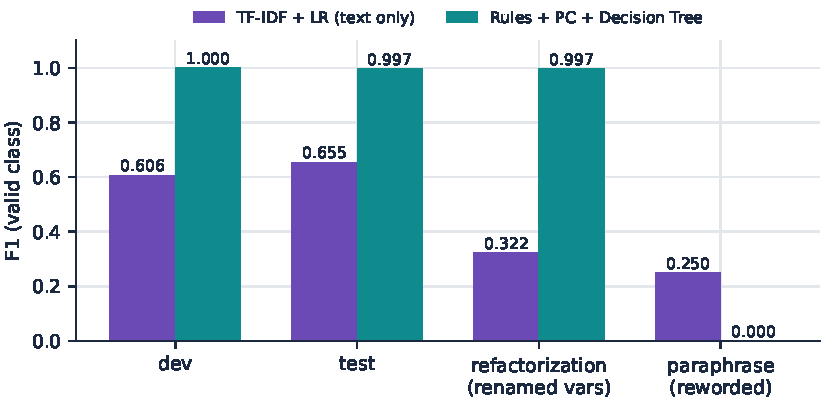
\includegraphics[width=0.86\linewidth]{figures/fig_robustness.pdf}
\caption{The text-only model halves its score when variables are renamed; the neuro-symbolic pipeline does not move.
Both fail on reworded hypotheses, for different reasons (\cref{sec:errors}).}
\label{fig:robust}
\end{figure}

\Cref{tab:main} and \cref{fig:robust} show three things:
\begin{itemize}
  \item \textbf{In distribution}, the pipeline is near-perfect (0.997 vs 0.655). TF-IDF reaches high recall only by
        flagging many claims as valid, so its precision is about 0.5.
  \item \textbf{Under renaming}, TF-IDF collapses from 0.655 to 0.322. Its recall falls from 0.94 to 0.24, the signature of the
        letter-order shortcut noted in \cref{sec:data}. Our features never see names, so the pipeline keeps 0.997.
  \item \textbf{On the original (buggy) labels} the pipeline still scores 0.949. The drop from 0.997 is consistent with
        the 18 test labels that the bug fix changed.
\end{itemize}

\begin{keybox}
Doing the causal reasoning symbolically turns a hard text-classification problem into an easy, interpretable one,
and makes the result immune to the variable-name shortcut that defeats text-only models.
\end{keybox}

% =====================================================================
\section{Graph Stage and Causal Queries}\label{sec:graph}

\subsection{Edge recovery}
From the classifier's direct-cause triples on the 21 test premises, the graph stage builds one DAG per premise. It
predicts \textbf{73 edges, all 73 correct}, against 73 gold edges: edge precision = recall = \textbf{1.00}.
\Cref{fig:graph} shows the largest test premise.

\begin{figure}[!htbp]
\centering
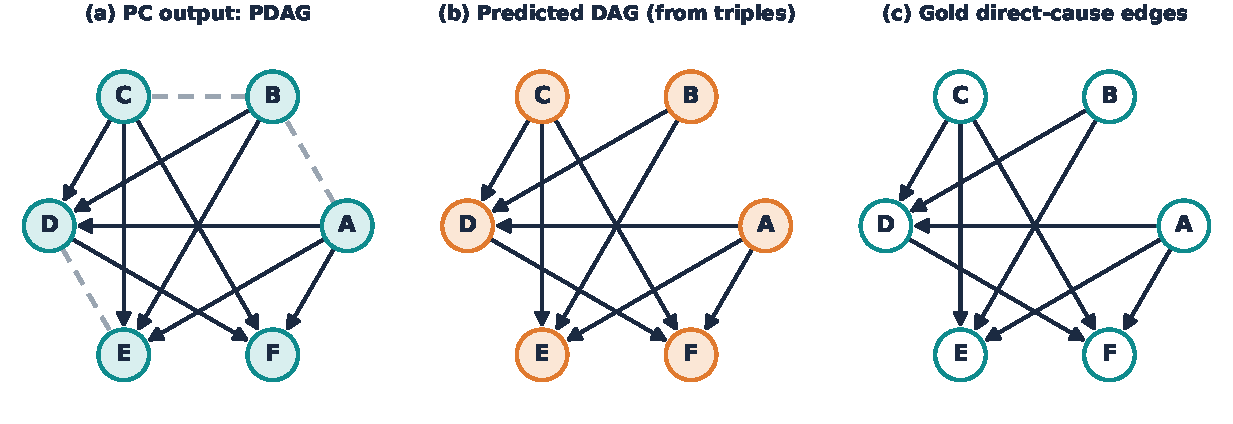
\includegraphics[width=0.95\linewidth]{figures/fig_graph.pdf}
\caption{A 6-variable test premise. (a) The PC output leaves three edges undirected. (b) The DAG assembled from
the classifier's accepted triples keeps only edges that are certain in every world. (c) It matches the gold direct-cause
edges exactly.}
\label{fig:graph}
\end{figure}

\paragraph{Acyclicity check.} Feeding the builder a contradictory candidate set,
A$\rightarrow$B (0.95), B$\rightarrow$C (0.90), C$\rightarrow$A (0.40), B$\rightarrow$B (0.30), keeps the first two and
rejects the cycle-closing C$\rightarrow$A and the self-loop. Text extraction alone cannot guarantee this; the graph
layer does, and it rejects the least confident edge first.

\subsection{Intervention queries}
The test premises yield \textbf{242 known queries} (spread over 14 of the 21 premises), and the Bayesian networks
answer \textbf{97.5\%} correctly (\cref{tab:queries}).

\begin{table}[!htbp]
\centering\small
\caption{Accuracy on known intervention queries ``does $\doop(X)$ change $Y$?''.}
\label{tab:queries}
\begin{tabular}{@{}lrr@{}}
\headrow \thead{Gold answer} & \thead{Queries} & \thead{Accuracy} \\
no effect (reverse direction or uncorrelated) & 153 & 1.000 \\
\rowcolor{mist} effect (direct or indirect cause) & 89 & 0.933 \\
\textbf{all} & \textbf{242} & \textbf{0.975} \\
\end{tabular}
\end{table}

All six misses are chains $X\rightarrow\cdots\rightarrow Y$ that pass through an edge whose direction the correlations
\emph{cannot identify}. The corresponding indirect claim is valid, because every equivalent DAG has \emph{some} path, but
no single direct edge on that path is certain. The conservative DAG leaves the edge out, so the network sees no path. This
is a limit of observational data (T2), not an extraction error. A Phase~2 option is to pass indirect triples to the graph
stage as path constraints.

\subsection{Why the Bayesian network matters: seeing vs doing}\label{sec:do}
\begin{figure}[!htbp]
\centering
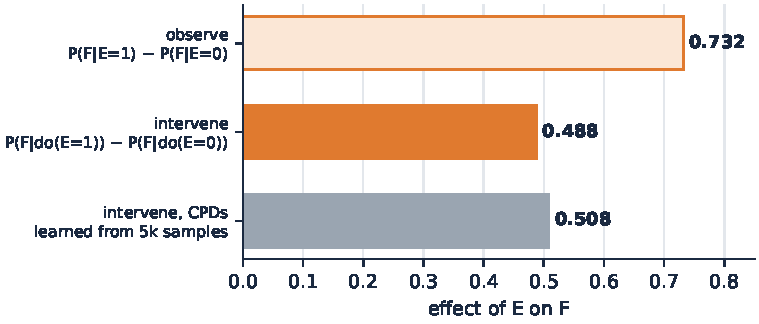
\includegraphics[width=0.62\linewidth]{figures/fig_do.pdf}
\caption{Test premise 20: E$\rightarrow$F, with A and D causing both. Observing E overstates its effect on F by 50\%.
Re-learning the tables from 5{,}000 simulated samples by maximum likelihood recovers the interventional effect (0.508 vs 0.488).}
\label{fig:do}
\end{figure}

\Cref{fig:do} makes theorem T4 concrete. Because A and D cause both E and F, seeing $E{=}1$ also signals that A or D is
probably active. The observational difference (0.732) is therefore much larger than the true causal effect of setting E (0.488).
A text extractor can say \emph{that} E causes F; only the network can say \emph{how much}, and keep that separate from
confounded association. The final bar shows that the network's probabilities are learnable: with real measurements (e.g.\ a
clinical table), \texttt{pgmpy} would fit them instead of using noisy-OR assumptions.

% =====================================================================
\section{Error Analysis and Limitations}\label{sec:errors}

\begin{figure}[!htbp]
\centering
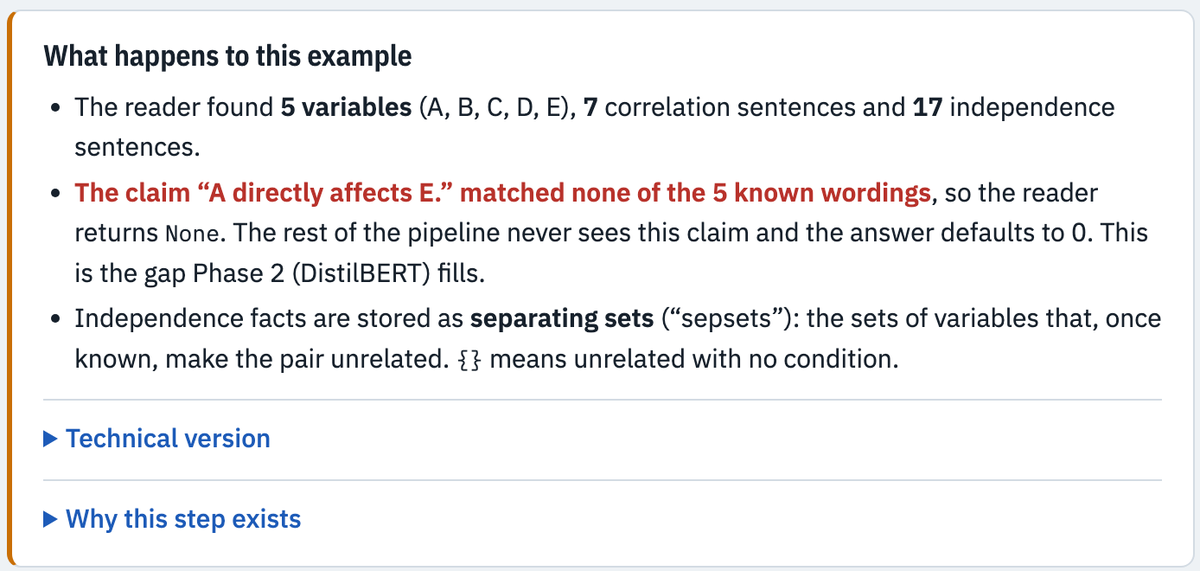
\includegraphics[width=0.66\linewidth]{figures/shot_tracer_paraphrase.png}
\caption{Screenshot from our pipeline tracer: a \emph{true} paraphrased claim (``A directly affects E.'') matches none of
the five known templates, so the language layer returns nothing and the claim defaults to ``not valid''.}
\label{fig:para}
\end{figure}

\begin{itemize}
  \item \textbf{Paraphrase is the open gap.} The regex reader parses 100\% of dev, test and refactorization hypotheses but
        \textbf{0\%} of paraphrased ones (\cref{fig:para}). The reasoning layer is never reached, so F1 = 0. TF-IDF does not
        fail outright, but at 0.25 it is barely useful. This is exactly the ``language understanding'' half of the brief, and it is
        what Phase~2 addresses.
  \item \textbf{Shortcut learning in text models.} TF-IDF's collapse under renaming shows that a model that only sees words
        learns dataset artefacts~\cite{gururangan2018,geirhos2020}. We expect fine-tuned transformers to be susceptible too, as
        Jin et al.\ report~\cite{jin2024corr2cause}, so Phase~2 will test renaming augmentation.
  \item \textbf{Synthetic, closed-world text.} Corr2Cause lists \emph{every} independence. Real abstracts list a few, often
        with hedging. The PC machinery would then need statistical tests or uncertainty-aware facts. PubMed remains an
        optional extension.
  \item \textbf{Illustrative probabilities.} Noisy-OR parameters are assumptions, not estimates. The ACE values show the
        mechanism, not real-world effect sizes (\cref{fig:do} shows the fitting path).
  \item \textbf{Small test set.} 21 premises (1{,}162 hypotheses) means one error moves F1 by about 0.003. We therefore also
        report dev and both robustness sets rather than relying on a single number.
\end{itemize}

% =====================================================================
\section{Reproducibility and Code Quality}\label{sec:repro}

The code is a small Python package with one module per pipeline stage, mirroring \cref{fig:pipeline}:

\begin{examplebox}
\footnotesize
\begin{tabularx}{\linewidth}{@{}>{\ttfamily}l@{\hspace{1.2em}}>{\leavevmode\color{slate}\raggedright\arraybackslash}X@{}}
src/causal\_nlp/parsing.py      & \textcolor{neural}{\textbf{Stage 1}}: text $\rightarrow$ facts / hypothesis triple \\
src/causal\_nlp/causal\_rules.py & \textcolor{symbolic}{\textbf{Stage 2}}: PC skeleton, v-structures, Meek R1--R3, equivalent DAGs, support \\
src/causal\_nlp/features.py     & \textcolor{symbolic}{\textbf{Stage 3}}: 23-feature table (cached per premise) \\
src/causal\_nlp/graph\_stage.py  & \textcolor{causal}{\textbf{Stage 5}}: acyclic DAG, noisy-OR BN, do-queries, edge metrics \\
src/causal\_nlp/data.py         & loaders, corrected labels, robustness sets (auto-download) \\
notebooks/01\_phase1\_ml\_pipeline.ipynb & executed Phase~1 deliverable (about 1--2 min on CPU) \\
tests/test\_pipeline.py         & 14 unit tests (parsing, PC, support, semantics, DAG, BN) \\
docs/pipeline\_visualiser.html  & interactive step-by-step pipeline tracer \\
results/                        & metrics and test triples saved for the Phase~2 comparison \\
\end{tabularx}
\end{examplebox}

\begin{itemize}
  \item \textbf{Deterministic.} Pinned dependencies, seed 42, and the official split. Re-running the notebook code for this
        report reproduced every number above exactly.
  \item \textbf{Tested.} All 14 unit tests pass (\code{pytest -q}). They cover, for example, a v-structure being found, a chain giving
        three equivalent DAGs, a cycle and a self-loop being rejected, and confounding making association larger than causation.
  \item \textbf{Swappable layer.} \code{build\_feature\_table(inputs, hypothesis\_parser=...)} accepts any parser, and
        \code{graph\_stage} consumes a plain triples table. Phase~2 plugs in without editing downstream code.
  \item \textbf{Explainable.} The pipeline tracer (\cref{fig:tracer}) follows real test examples through all nine stages, next to
        the exact source lines that process them, which also serves as viva preparation for every team member.
\end{itemize}

\begin{figure}[!htbp]
\centering
\begin{subfigure}[b]{0.56\linewidth}\centering
  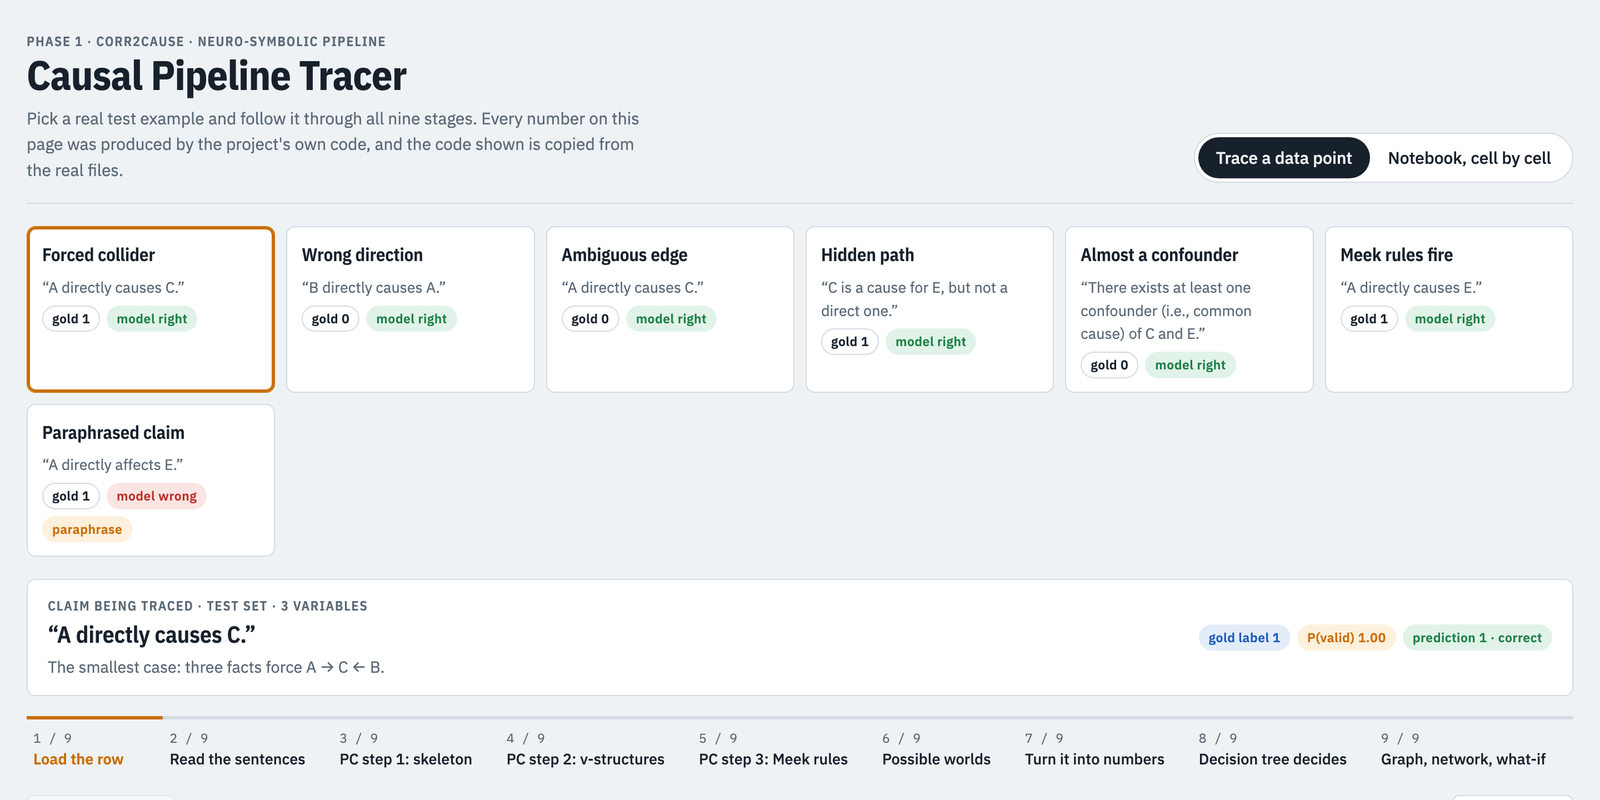
\includegraphics[width=\linewidth]{figures/shot_tracer_overview.png}
  \caption{Choosing a real example and the nine-stage timeline.}
\end{subfigure}\hfill
\begin{subfigure}[b]{0.4\linewidth}\centering
  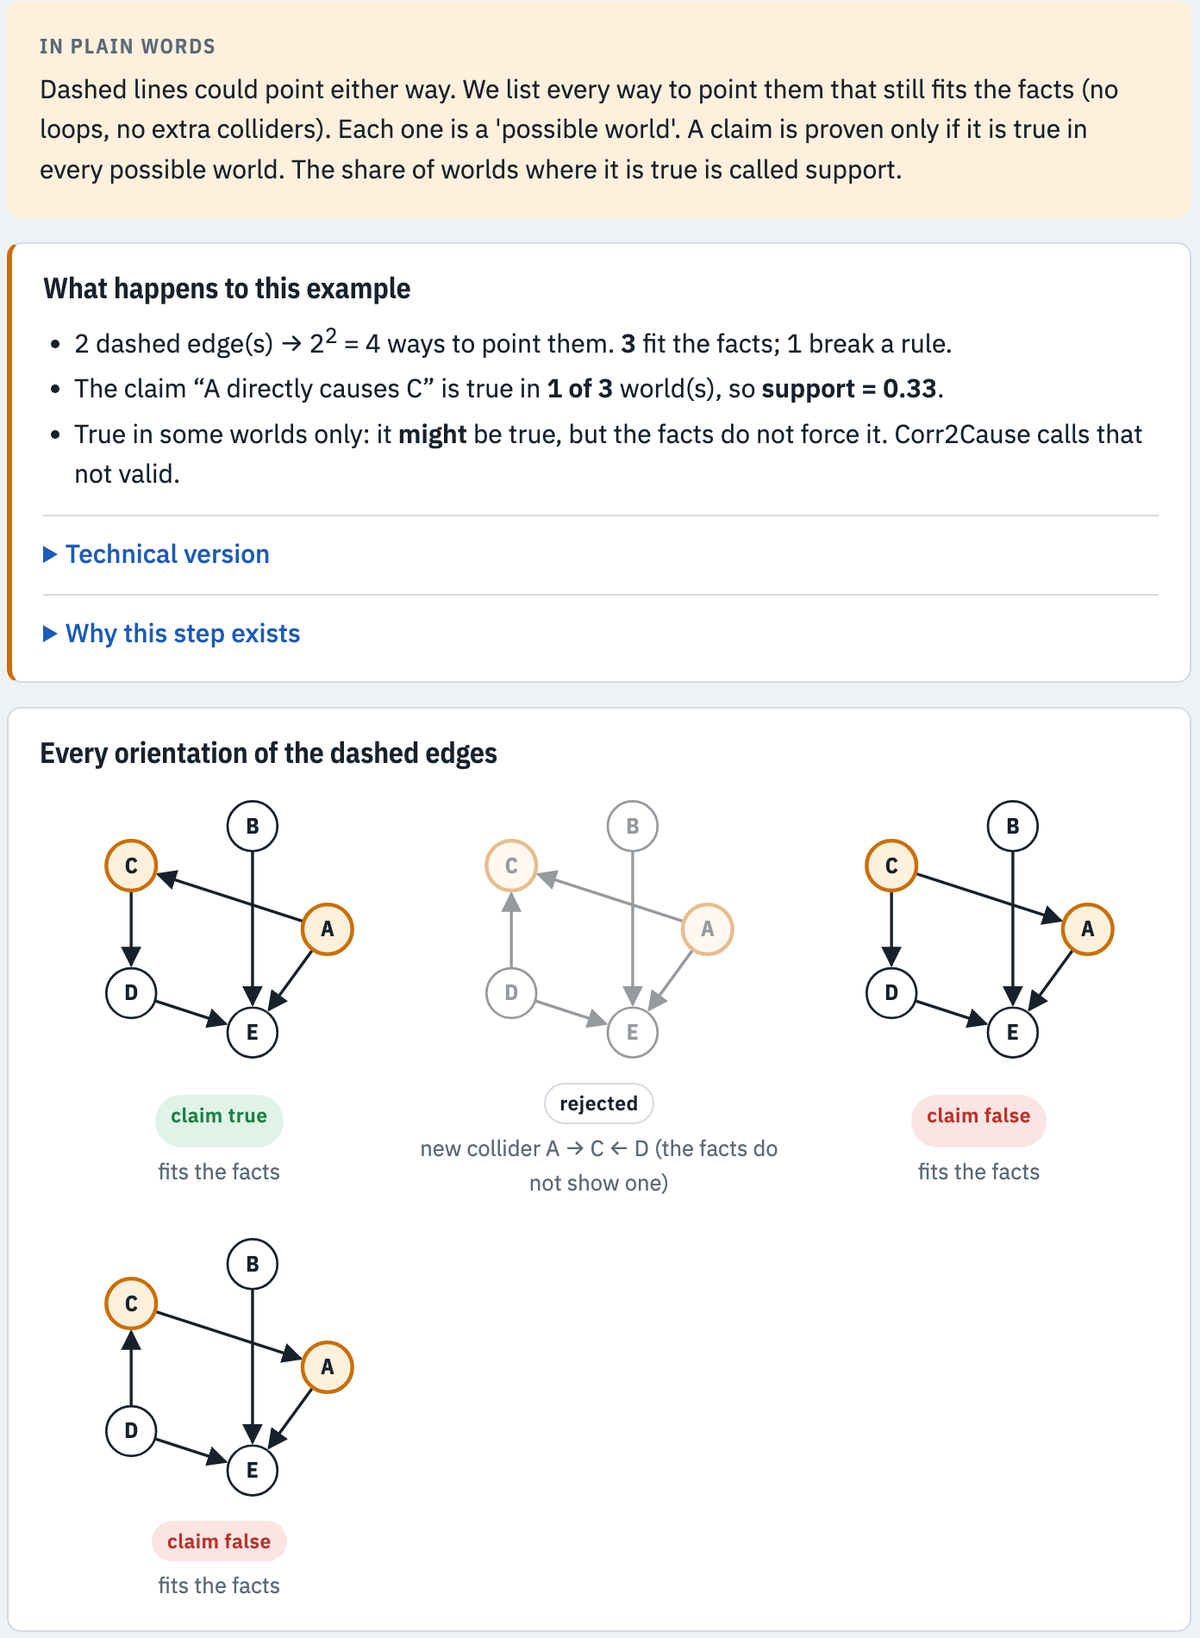
\includegraphics[width=\linewidth]{figures/shot_tracer_worlds.png}
  \caption{Stage 6: the ``possible worlds'' behind support = 1/3.}
\end{subfigure}
\captionsetup{justification=raggedright,singlelinecheck=false}
\caption{Screenshots of the interactive tracer \texttt{docs/pipeline\_visualiser.html}, which \texttt{tools/build\_visualiser.py} generates from the project's own code and outputs.}
\label{fig:tracer}
\end{figure}

% =====================================================================
\section{Road to Phase 2}\label{sec:phase2}

Phase~2 keeps the reasoning and graph layers and the evaluation code fixed, and adds two transformer systems, each paired
with its Phase~1 counterpart (\cref{tab:phase2}).

\begin{table}[!htbp]
\centering\small
\caption{Planned comparison grid. Same splits, same metrics, same graph stage.}
\label{tab:phase2}
\begin{tabularx}{\linewidth}{@{}l>{\raggedright}X>{\raggedright\arraybackslash}X@{}}
\headrow & \thead{Text only (no reasoning layer)} & \thead{Language layer + reasoning layer} \\
\textbf{ML (Phase 1)} & TF-IDF + LR & Rules + PC + Decision Tree \\
\rowcolor{neuralT}\textbf{DL (Phase 2)} & \textbf{2A}: DistilBERT end-to-end classifier, $\pm$ variable-renaming augmentation &
  \textbf{2B}: DistilBERT hypothesis parser $\rightarrow$ PC + Decision Tree (hybrid) \\
\end{tabularx}
\end{table}

\begin{itemize}
  \item \textbf{2A} reads \code{[CLS] hypothesis [SEP] premise [SEP]} (max 512 tokens, truncating the premise tail) and is
        expected to beat TF-IDF in distribution, but to inherit the renaming weakness unless names are augmented.
  \item \textbf{2B} is the hybrid the brief rewards: DistilBERT only maps a hypothesis to \code{(relation, x, y)}. It is trained
        on template hypotheses plus our own hand-written paraphrases, with the official paraphrase wordings held out. Paraphrase
        F1 should rise from 0 towards the parser's accuracy while in-distribution and renaming scores stay at Phase~1 levels.
  \item Final table: dev / test / refactorization / paraphrase F1, edge precision and recall, query accuracy, training time and
        parameter count, plus an error analysis of 20 failures per DL system.
\end{itemize}

% =====================================================================
\section{Conclusion}
Phase~1 shows that separating language from reasoning is effective. A small set of regex rules, a faithful
implementation of the PC algorithm, and a depth-4 decision tree solve Corr2Cause almost perfectly (test F1 0.997). They
are unaffected by variable renaming, recover every gold cause edge, and answer 97.5\% of intervention queries. The
Bayesian network adds what extraction cannot: guaranteed acyclicity, quantified effects, and a principled distinction
between observing and intervening. The remaining weakness is purely linguistic. When the wording changes, the rules
cannot read the claim, so Phase~2 brings in DistilBERT for exactly that job while the reasoning layer stays as it is.

% =====================================================================
\section*{Team Contributions}
\addcontentsline{toc}{section}{Team Contributions}
\begin{table}[!htbp]
\centering\small
\begin{tabularx}{\linewidth}{@{}lX@{}}
\headrow \thead{Member} & \thead{Primary responsibility} \\
\MemberA & Project lead: pipeline design, graph stage, Bayesian network and do-queries; pipeline tracer; report (\cref{sec:graph,sec:repro}) \\
\rowcolor{mist} \MemberB & Data loading, label correction, leakage checks and EDA (\cref{sec:data}) \\
\MemberC & Feature engineering, classifiers and ablation (\cref{sec:results}) \\
\rowcolor{mist} \MemberD & Reasoning layer: PC algorithm, Meek rules, equivalent DAGs and support; graph-stage tests (\cref{sec:theory}) \\
\MemberE & Language layer: entity schema and regex extractor; robustness sets (\cref{sec:method}) \\
\end{tabularx}
\end{table}

% =====================================================================
\begingroup
\small
\renewcommand{\refname}{References}
\begin{thebibliography}{99}\setlength{\itemsep}{2pt}
\bibitem{pearl1988} J.~Pearl, \emph{Probabilistic Reasoning in Intelligent Systems: Networks of Plausible Inference}. Morgan Kaufmann, 1988.
\bibitem{devlin2019} J.~Devlin, M.-W.~Chang, K.~Lee, and K.~Toutanova, ``BERT: Pre-training of deep bidirectional transformers for language understanding,'' in \emph{Proc.\ NAACL-HLT}, 2019, pp.~4171--4186.
\bibitem{jin2024corr2cause} Z.~Jin, J.~Liu, Z.~Lyu, S.~Poff, M.~Sachan, R.~Mihalcea, M.~Diab, and B.~Sch\"olkopf, ``Can large language models infer causation from correlation?'' in \emph{Proc.\ ICLR}, 2024.
\bibitem{spirtes2000} P.~Spirtes, C.~Glymour, and R.~Scheines, \emph{Causation, Prediction, and Search}, 2nd~ed. MIT Press, 2000.
\bibitem{meek1995} C.~Meek, ``Causal inference and causal explanation with background knowledge,'' in \emph{Proc.\ UAI}, 1995, pp.~403--410.
\bibitem{verma1990} T.~Verma and J.~Pearl, ``Equivalence and synthesis of causal models,'' in \emph{Proc.\ UAI}, 1990, pp.~255--270.
\bibitem{pearl2009} J.~Pearl, \emph{Causality: Models, Reasoning, and Inference}, 2nd~ed. Cambridge University Press, 2009.
\bibitem{sanh2019} V.~Sanh, L.~Debut, J.~Chaumond, and T.~Wolf, ``DistilBERT, a distilled version of BERT: smaller, faster, cheaper and lighter,'' arXiv:1910.01108, 2019.
\bibitem{khoo2000} C.~S.~G.~Khoo, S.~Chan, and Y.~Niu, ``Extracting causal knowledge from a medical database using graphical patterns,'' in \emph{Proc.\ ACL}, 2000, pp.~336--343.
\bibitem{girju2003} R.~Girju, ``Automatic detection of causal relations for question answering,'' in \emph{Proc.\ ACL Workshop on Multilingual Summarization and Question Answering}, 2003, pp.~76--83.
\bibitem{gururangan2018} S.~Gururangan, S.~Swayamdipta, O.~Levy, R.~Schwartz, S.~Bowman, and N.~A.~Smith, ``Annotation artifacts in natural language inference data,'' in \emph{Proc.\ NAACL-HLT}, 2018, pp.~107--112.
\bibitem{geirhos2020} R.~Geirhos, J.-H.~Jacobsen, C.~Michaelis, R.~Zemel, W.~Brendel, M.~Bethge, and F.~A.~Wichmann, ``Shortcut learning in deep neural networks,'' \emph{Nature Machine Intelligence}, vol.~2, pp.~665--673, 2020.
\bibitem{kiciman2023} E.~K{\i}c{\i}man, R.~Ness, A.~Sharma, and C.~Tan, ``Causal reasoning and large language models: Opening a new frontier for causality,'' arXiv:2305.00050, 2023.
\bibitem{garcez2023} A.~d'Avila Garcez and L.~C.~Lamb, ``Neurosymbolic AI: The 3rd wave,'' \emph{Artificial Intelligence Review}, vol.~56, pp.~12387--12406, 2023.
\bibitem{ankan2015} A.~Ankan and A.~Panda, ``pgmpy: Probabilistic graphical models using Python,'' in \emph{Proc.\ SciPy}, 2015, pp.~6--11.
\bibitem{corr2causecorrected} Corr2Cause corrected labels, Hugging Face dataset \texttt{zluke/corr2cause-corrected}, \url{https://huggingface.co/datasets/zluke/corr2cause-corrected}.
\end{thebibliography}
\endgroup

\end{document}
